\subsection{Smart Contracts}
\label{subsec:02_smart_contracts}

\textbf{Length: around 2 pages}

This section will look at the concept of smart contracts in the concept of ethereum.
Ethereum is a blockchain ''with built in programming language'', or in other words a ''consensus-based globally executed virtual machine''. 
The ethereum project started in 2015 and has gained popularity since then. In fact, it is second place in terms of market capitalization according to coinmarketcap.com, right after bitcoin and followed by ripple.

Nodes in the ethereum network make up the EVM (Ethereum virtual machine). Smart contracts are written in the programming language solidity. They get then compiled to bytecode that the EVM can understand.
Once deployed on the blockchain, the code cannot be changed. Deploying smart contracts means mining them into the blockchain, thus deploying smart contract costs gas like every other transactions. Once they are there, they are part of the blockchain history.
Every smart contract on the blockchain lives at an address where the contracts exposed functions and variables can interacted with. Solidity is an object-oriented programming language and comes with known modifiers such as ``public'' and ``private'' and more.
It is perfectly possible to write smart contracts that do nothing sensible, or even nothing at all, e.g. smart contract with a private state variable without getters or setters.
Such a contract would do nothing but sit on the blockchain doing nothing. Smart contracts can inherit from smart contracts and interact with other smart contracts. 
Smart contracts can even be sent ether to. Sending ether to a smart contract that does not provide functionality to retrieve those ethers means they are lost forever in the contract.
This is crucial especially when designing contracts that implement business logic or any contracts for that matter. Smart contracts should be reviewed and audited carefully and tested for vulnerabilities else its weaknesses can be exploited like in the infamous``DOA' attack.

Every transaction on the blockchain costs gas. Gas is expressed in ether. The miner that mines a transaction collects the gas associated with it, thus gas serves as an incentive for miners to mine and contribute to the network. There is a defined set of operations with their respective gas costs in the etherum yellow paper.
Figure \ref{fig:smart_contract_fees} shows and excerpt of those costs.

\begin{figure}[ht!]
  \begin{center}
  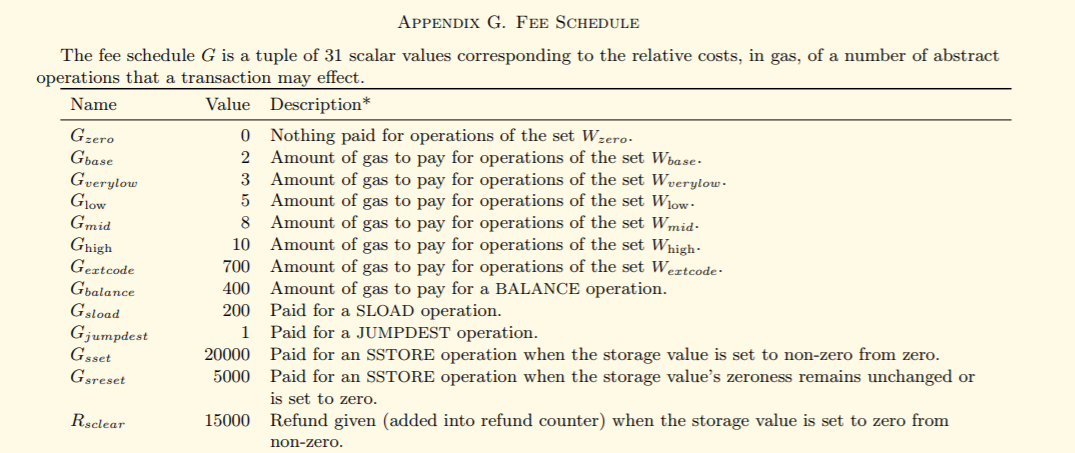
\includegraphics[scale=0.6]{Talk7/img/smart_contracts/gas-fees}
 	\end{center}
  \caption{Smart contract fees from ethereum yellow paper}
 	\label{smart_contract_fees}
\end{figure}

Miners will generally prioritize transactions with a higher gas fee. The total gas fee to be paid is calculated by the gas price times the amount of gas to use. If the gas price for a transaction is set high, the transaction will be mined to the blockchain faster. If on the other hand the price is set low, miners will choose to mine other transactions first
before mining transactions with a lower price. How high the gas price is is determined by the market. During peak network traffic gas price will be high because more people want their transaction to go through driving prices up. When the network is more relaxed prices drop.
A transaction has a gas limit that can be set. This is to indicate the maximum amount of gas a transaction can use up before it is aborted. The gas limit times the gas price is maximum amount the issuer is willing to pay for a transaction. In case of an endless loop, the execution will only last as long until the gas limit is used up.
If the gas limit is too little, the computation will run out ouf gas before it is finished it will be reverted and the gas paid will be lost. If the gas limit is higher than the amount of gas actually used, the remaining gas will be refunded to the sender of the transaction. 
Miners can only put so many transactions in a block that block gas limit is not exceeded. This is also not a fixed value as miners can vote with each block to increase or decrease the block gas limit by a certain amount. Block gas limit serves to keep propagation of blocks and transaction time low by essentially limiting the size of the blocks.

The following list sums up the key terms mentioned above
\begin{itemize}
  \item {gas:}
  \item {gas prize:}
  \item {gas limit:}
  \item {transaction fee:}
  \item {block gas limit:}
  
\end{itemize}

In fact, not all smart contract interaction costs gas. Functions that do not modify the state of a contract, and hence the blockchain, do not need to be mined by a miner.
Calling those functions will still use gas, because every operation in the EVM uses gas, but that gas is refunded immediately as calling those functions do no not result in a transaction.
In solidity those functions have the modifier ``pure'' or ``view''. Functions denoted with ``pure'' don't even read state variables. Both those functions can be run on a single node in the EVM and 
nothing has to be propagated to the network thus no transaction has to be mined into the blockchain and no gas fee has to be paid.

%% Copyright 2017 Sergei Tikhomirov, MIT License
% https://github.com/s-tikhomirov/solidity-latex-highlighting/

\usepackage{listings, xcolor}

\definecolor{verylightgray}{rgb}{.97,.97,.97}

\lstdefinelanguage{Solidity}{
	keywords=[1]{anonymous, assembly, assert, balance, break, call, callcode, case, catch, class, constant, continue, constructor, contract, debugger, default, delegatecall, delete, do, else, emit, event, experimental, export, external, false, finally, for, function, gas, if, implements, import, in, indexed, instanceof, interface, internal, is, length, library, log0, log1, log2, log3, log4, memory, modifier, new, payable, pragma, private, protected, public, pure, push, require, return, returns, revert, selfdestruct, send, solidity, storage, struct, suicide, super, switch, then, this, throw, transfer, true, try, typeof, using, value, view, while, with, addmod, ecrecover, keccak256, mulmod, ripemd160, sha256, sha3}, % generic keywords including crypto operations
	keywordstyle=[1]\color{blue}\bfseries,
	keywords=[2]{address, bool, byte, bytes, bytes1, bytes2, bytes3, bytes4, bytes5, bytes6, bytes7, bytes8, bytes9, bytes10, bytes11, bytes12, bytes13, bytes14, bytes15, bytes16, bytes17, bytes18, bytes19, bytes20, bytes21, bytes22, bytes23, bytes24, bytes25, bytes26, bytes27, bytes28, bytes29, bytes30, bytes31, bytes32, enum, int, int8, int16, int24, int32, int40, int48, int56, int64, int72, int80, int88, int96, int104, int112, int120, int128, int136, int144, int152, int160, int168, int176, int184, int192, int200, int208, int216, int224, int232, int240, int248, int256, mapping, string, uint, uint8, uint16, uint24, uint32, uint40, uint48, uint56, uint64, uint72, uint80, uint88, uint96, uint104, uint112, uint120, uint128, uint136, uint144, uint152, uint160, uint168, uint176, uint184, uint192, uint200, uint208, uint216, uint224, uint232, uint240, uint248, uint256, var, void, ether, finney, szabo, wei, days, hours, minutes, seconds, weeks, years},	% types; money and time units
	keywordstyle=[2]\color{teal}\bfseries,
	keywords=[3]{block, blockhash, coinbase, difficulty, gaslimit, number, timestamp, msg, data, gas, sender, sig, value, now, tx, gasprice, origin},	% environment variables
	keywordstyle=[3]\color{violet}\bfseries,
	identifierstyle=\color{black},
	sensitive=false,
	comment=[l]{//},
	morecomment=[s]{/*}{*/},
	commentstyle=\color{gray}\ttfamily,
	stringstyle=\color{red}\ttfamily,
	morestring=[b]',
	morestring=[b]"
}

\lstset{
	language=Solidity,
	backgroundcolor=\color{verylightgray},
	extendedchars=true,
	basicstyle=\footnotesize\ttfamily,
	showstringspaces=false,
	showspaces=false,
	numbers=left,
	numberstyle=\footnotesize,
	numbersep=9pt,
	tabsize=2,
	breaklines=true,
	showtabs=false,
	captionpos=b
}
	

\begin{lstlisting}[language=Solidity]
  pragma solidity 0.4.16;
  
  contract TestContract {
      
    string private myString = "foo";
    
    function getString() constant returns (string) {
        return myString;
    }
    
    function setString (string _string) {
        myString = _string;
    }
  }
  \end{lstlisting}